\section{Análise de métodos de atribuição de estrutura secundária}

Diferentemente de outros métodos de predição de estrutura secundária que utilizaram os resultados de atribuição provenientes de apenas um método, em geral o DSSP, nós optamos por utilizar os resultados de um concenso entre quatro métodos. Consequentemente, é importante analizar como esses métodos diferem entre si.

As diferenças entre as metologias de atribuição foram previamente discutidas na seção \ref{section:metodos_atribuicao}. Nesta seção, analisaremos as diferenças nas estruturas secundárias atribuídas aos resíduos.



\begin{figure}
  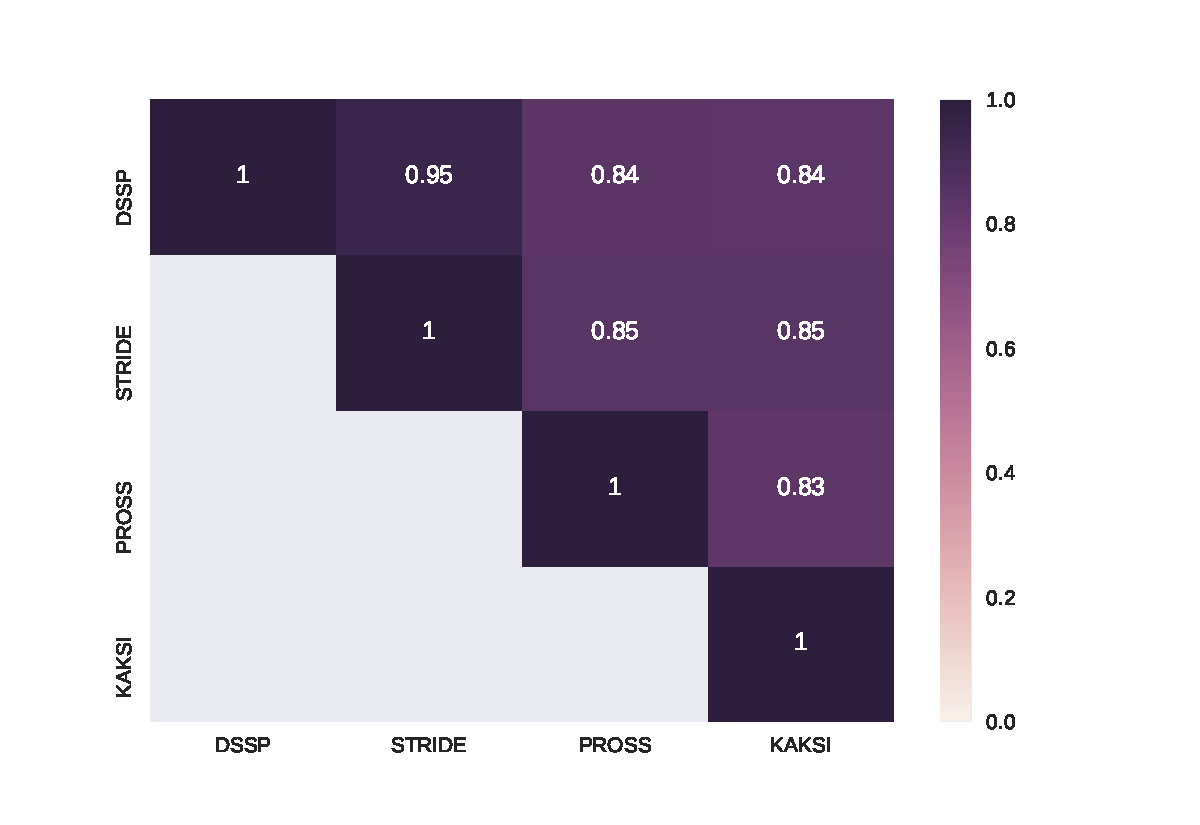
\includegraphics[width=\linewidth]{../figures/comparacao_metodos_atribuicao.pdf}
  \caption{Similaridade entre os métodos de atribuição de estruturas secundárias.}
  \label{fig:comparacao_metodos_atribuicao}
\end{figure}